\documentclass[deutsch]{llncs}
\usepackage{multirow, cellspace}
\usepackage{microtype}
\usepackage{tabularx}
\usepackage{ltablex}
\usepackage{amssymb}
\usepackage{amsmath}
\usepackage[utf8]{inputenc} %Umlaute
\usepackage{amssymb}
\usepackage{upgreek}
\usepackage{graphicx}
\usepackage{amsmath}
\usepackage{array}
\usepackage{gensymb}
\usepackage{enumerate}

% subfigure
\usepackage{caption}
\usepackage{subcaption}
%

\usepackage{adjustbox}

\renewcommand{\arraystretch}{1.5}
\renewcommand{\labelenumi}{\Alph{enumi}.}
\setlength{\jot}{10pt}

\begin{document}

\title{Intelligente Sehsysteme - Übungsblatt 7}


\author{Hendrik Walther, Jan Konrad}
\institute{}
\maketitle
\setcounter{section}{1}
\section{Korrespondierende Kosinus-Funktionen}
Für zwei an $N$ Orten abgetastete Funktionen $\cos(u_1\cdot n)$
und $\cos(u_2\cdot n)$ mit $ \frac{u_1}{u_0} = N - \frac{u_2}{u_0}$,
gilt: $\cos(u_1\cdot n)=\cos(u_2\cdot n)$ \\

\begin{equation}
	\label{cos1}
	\forall n \in \mathbb{Z}: \cos(x + 2\pi n) = \cos(x)
\end{equation}
\begin{equation}
	\label{cos2}
	\cos(-x ) = \cos(x)
\end{equation} \\
\begin{equation}
	\label{u1}
	\begin{alignedat}{3}
		& \frac{u_1}{u_0} & = & N - \frac{u_2}{u_0} \\
		\iff                                   & u_1             & = & N \cdot u_0 - u_2   \\
		\stackrel{u_0 = \frac{2 \pi}{N}}{\iff} & u_1             & = & 2\pi - u_2          \\
	\end{alignedat}
\end{equation} \\

\begin{equation}
	\begin{aligned}
		                                  & \cos(u_1\cdot n)            \\
		\stackrel{\text{(\ref{u1})}}{=}   & \cos(2\pi  n - u_2 \cdot n) \\
		\stackrel{\text{(\ref{cos1})}}{=} & \cos( - u_2 \cdot n)        \\
		\stackrel{\text{(\ref{cos2})}}{=} & \cos( u_2 \cdot n)          \\
	\end{aligned}
\end{equation}
\newpage
\setcounter{section}{5}
\section{ITB: Gauß-Pyramide}
\begin{figure}
	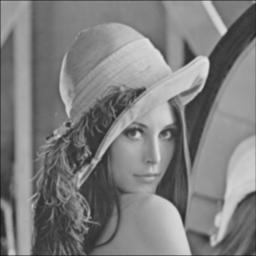
\includegraphics[]{A6/1.jpg}
	
\includegraphics[]{A6/2.jpg}
	
\includegraphics[]{A6/3.jpg}
	
\includegraphics[]{A6/4.jpg}
	
\includegraphics[]{A6/5.jpg}
	
\includegraphics[]{A6/6.jpg}
	
\includegraphics[]{A6/7.jpg}
	\caption{Reduce}
\end{figure}

\begin{figure}
	\centering
	\begin{subfigure}{.49\textwidth}
		\centering
		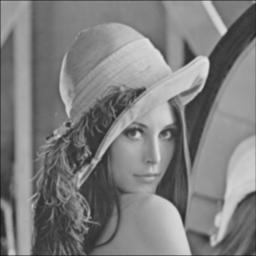
\includegraphics[width=.99\linewidth]{A6/1.jpg}
		
\includegraphics[width=.99\linewidth]{A6/2.jpg}
		\caption{Reduce}
	\end{subfigure}
	\begin{subfigure}{.49\textwidth}
		\centering
		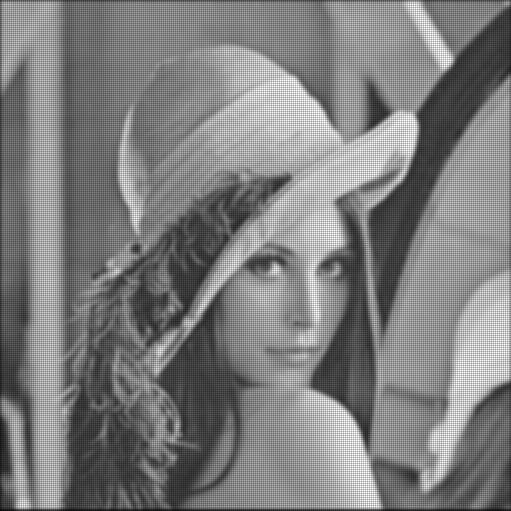
\includegraphics[width=.99\linewidth]{A6/expand1.jpg}
		
\includegraphics[width=.99\linewidth]{A6/expand2.jpg}
		\caption{Expand}
	\end{subfigure}
\end{figure}

\end{document}
